\hypertarget{rgb-ux56e0ux679cux5e72ux9884}{%
\section{RGB 因果干预}\label{rgb-ux56e0ux679cux5e72ux9884}}

\hypertarget{rgb-ux56e0ux679cux5e72ux9884-1}{%
\subsection{RGB 因果干预}\label{rgb-ux56e0ux679cux5e72ux9884-1}}

\begin{figure}
\centering
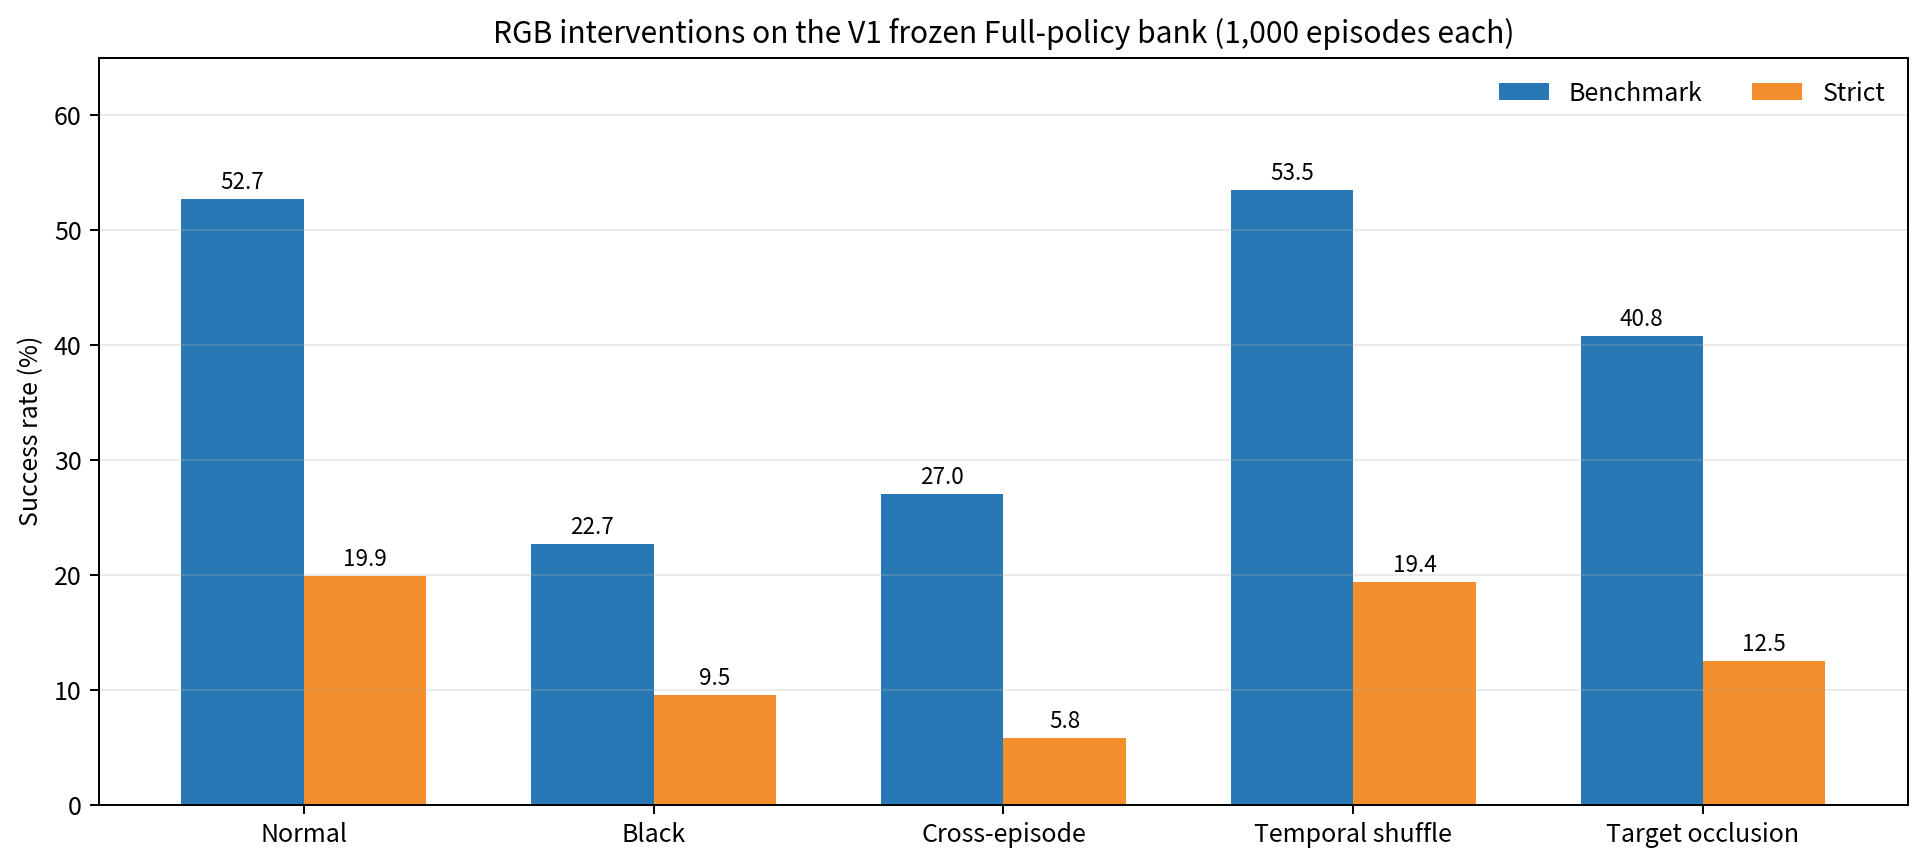
\includegraphics[width=\linewidth]{figures/04_visual_interventions.png}
\caption{视觉干预结果}
\end{figure}

\textbf{图 4｜V1 视觉干预。} 每种条件评测相同 5 个训练 seed，共 1,000 episodes；Normal 为冻结 Full policy，Benchmark 表示任意时刻 entry，Strict 表示末 20 步连续成功。图内所有柱属于同一个 V1 干预协议，没有与后续 100/300/200-episode bank 连线。

Normal RGB 下为 52.7\% Benchmark、19.9\% Strict。RGB 全黑后降至 22.7\% / 9.5\%，跨 episode 打乱降至 27.0\% / 5.8\%，遮挡绿色目标笔降至 40.8\% / 12.5\%。这三类干预都不改变 proprioception，却明显损害闭环，因此可以排除``策略完全忽略 RGB，只靠手部状态''的解释，也说明目标外观是有效视觉线索。

然而，4 帧时间顺序打乱后仍为 53.5\% / 19.4\%，与 Normal 基本相同。这不是视觉无用，而是更细的结论：原 CNN 主要使用静态外观或近似集合信息，没有可靠提取帧顺序、角速度和接触动态。它解释了为何基础视觉策略能到达目标，却容易在 hold 阶段退出，也为后续改用显式因果 GRU 提供了直接证据。
